The library consists of two main layers on the client side. An upper layer
to implement the RVM-specific logic and a lower-layer remote memory (RMEM)
backend to implement low-level transport and atomicity. This relationship is
described in Figure \ref{fig:lasagna}. This modularization allows for a number of
different backends to be tried independently of user code and the RVM layer.
This enhances portability and simplifies future efforts to improve performance
or semantics.

\begin{figure}[t]
\begin{center}
\resizebox{\columnwidth}{!}{%
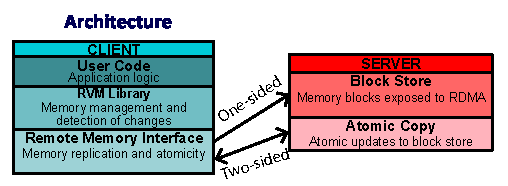
\includegraphics[scale=0.80]{lasagna.pdf}
}
\end{center}
\caption{RVM lasagna diagram}
\label{fig:lasagna}
\end{figure}

\subsection{The RVM API}

The RVM layer is responsible for implementing the custom allocator and
identifying changes to memory. It is also responsible for tracking commit
points.

\subsubsection{The Block Table}
The RVM layer thinks in terms of \emph{blocks}, fixed-sized regions of
memory that are persisted atomically. Most functionality is based around the
\emph{block table}, a persistent data structure that keeps track of each
allocated block in the system. This table is replicated using the same
mechanism as any other recoverable memory. Like a filesystem master boot record,
the first page of the block table is always stored with a constant identifier
in the RMEM layer. After that, the block table is self-describing and can be
recovered using the mechanisms described below.

Each entry in the block table contains a local address where the active block
lives on the client and a remote identifier that can be used to identify the
block in the RMEM layer. 

\subsubsection{Initialization and Recovery Procedure}

When \verb|rvm_cfg_create()| is called the first time, it initializes the block
table to an empty state and persists it in the RMEM layer. When recovering,
\verb|rvm_cfg_create()| fetches the first block of the block table from the
RMEM layer. The block table is walked from start to finish, fetching each block
as it goes. Even if the block table takes up multiple blocks, each one is
fetched in order, ensuring that all data can be found eventually. When RVM
fetches a remote block, it must ensure that it is loaded to the same address it
was at before failure, otherwise pointers in the data would no longer be valid.
The original address is read from the block table and then allocated using the
\emph{mmap()} system call. To ensure that these addresses are always available,
RVM requires that any OS address space layout randomization be disabled, and
that \verb|rvm_cfg_create()| be called before any other local allocations.

\subsubsection{Allocation}

To ensure that memory is recoverable, the user must allocate it using a special
\verb|rvm_alloc()| function. The \verb|rvm_alloc()| function allocates memory
both locally and on the remote node. Any modifications to the local pages
allocated by \verb|rvm_alloc()| are automatically detected and copied to the
remote node at commit time. Detection is achieved through the use of
\emph{mprotect()}, a Linux system call that can be used to make the application
take an interrupt whenever a page is written. Our custom interrupt handler
then marks the page as changed, removes the memory protection and returns. This
means that RVM needs to be involved only in the first modification to a page.

\subsubsection{Marking a Point of Consistency}

The user is required to identify points in their code where the state of
recoverable memory is considered \"consistent\". This means that recovery is
possible from that particular state. \verb|rvm_txn_commit()| can be called at
these points to ensure that memory is atomically persisted. Upon entering
\verb|rvm_txn_commit()|, RVM goes through the list of changed pages and copies
them to a shadow page in the RMEM layer. This ensures that a consistent version
of memory is always available, even if the client crashes during checkpointing.
When all the pages have been copied, an \verb|atomic_commit()| function
(provided by the RMEM layer) is called to persist the changes.



\subsection{The Remote Memory Layer}

Underlying the RVM API is the remote memory (RMEM) layer, which provides the
basic operations that RVM uses to communicate with the backing data store.
The essential operations in the RMEM layer are \texttt{malloc()},
\texttt{free()}, \texttt{put()}, \texttt{get()}, and \texttt{atomic\_commit()}.

The \texttt{malloc()} function allocates memory in the backing store.
The function arguments include the number of bytes to allocate as well as
a unique tag that is associated with that memory region. If the tag has not
already been taken, \texttt{malloc()} allocates a new memory region and returns
the starting address. If a memory region with that tag already exists, the
starting address of the previously allocated region is returned.

The \texttt{free()} function takes a tag as its argument and frees the memory
region associated with that tag.

There are also \texttt{multi\_malloc()} and \texttt{multi\_free()} functions
which allocate and free multiple memory blocks. Depending on the backend,
these functions might coalesce \texttt{malloc()} and \texttt{free()} requests
in order to decrease the number of round trips to the backing store.

The \texttt{put()} and \texttt{get()} functions copy data to and from the
backing store, respectively. These operations are not atomic, so the RVM
layer always performs puts and gets onto a shadow page and then copies the
data to the real page using \texttt{atomic\_commit()}.

As mentioned before, \texttt{atomic\_commit()} takes an array of source tags
and an array of destination tags. It instructs the server to copy the data
in the source memory regions to the destination regions. This copying is
done atomically, so there is no danger of only a portion of the pages
being copied due to the client crashing.


\subsection{Infiniband Backend}

Our primary backend uses Infiniband Remote Direct Memory Access (RDMA) to talk
to a server managing a large pool of memory. At startup, the remote memory
server maps in a large block of system memory. The server then listens for
connections over the Infiniband fabric. When a client connects, the server
pins the memory in the page table and registers it with the infiniband drivers.
Registering with the infiniband drivers provides a local key and a remote key.
The server transmits the remote key and starting address to the client.
This allows the client to perform one-sided RDMA operations to the remote
memory without the server's mediation.

The \texttt{put()} and \texttt{get()} commands are implemented using one-sided
RDMA writes and reads. The other commands are implemented using two-sided sends
and receives. For these commands, the client and server each allocate two
message structs: one for sends, and one for receives. In a two-sided
transmission, the recipient first posts a receive request to the Infiniband
driver. This receive request specifies the local key and address of the receive
struct. When the sender posts a corresponding send request using the local key
and address of its send struct, the infiniband drivers copy the data from the
sender's send struct to the recipient's receive struct and notify sender and
recipient of the operation.

\begin{figure}
    \includegraphics[width=0.9\linewidth]{ib-backend-arch.pdf}
    \caption{IB Backend Architecture}
    \label{fig:ib-backend-arch}
\end{figure}

\subsubsection{Allocation}

The \texttt{malloc()} operation is implemented by sending an ALLOC request to
the server. When it receives this request, the server will allocate a block of
memory form the memory pool and mark it with the given tag.  The server then
sends a MEMRESP message back to the client containing the starting address of
the allocated block.

The \texttt{free()} operation is implemented by sending a TXN\_FREE request to
the server. A key feature of the IB backend is that the server does not
immediately perform a free operation when it receives the TXN\_FREE message.
Instead, it puts the free operation in a queue, which will be processed during
an atomic commit. This way, the free operation is transactional. Once the
server receives the message and queues the free operation, it sends a TXN\_ACK
message back to the client, allowing the client to send another command.

There are also MULTI\_ALLOC and MULTI\_TXN\_FREE requests which can encode up
to 20 allocation or free requests (this number if configurable at compile
time). The server responds to a MULTI\_ALLOC request with a MULTI\_MEMRESP
response, which contains an array of addresses, one for each tag in the
MULTI\_ALLOC request. The server responds to MULTI\_TXN\_FREE with a TXN\_ACK.

\subsubsection{Commit}

The \texttt{atomic\_commit()} operation involves two different message types.
The first is the MULTI\_TXN\_CP message, which instructs the server to copy a
set of source blocks to a set of destination blocks. However, as with
TXN\_FREE, the copy does not occur immediately. When the client sends the
server a TXN\_GO request, the server performs all requested copies and frees.
In our failure model, we assume that the server will not crash. So even if the
client crashes after sending TXN\_GO, the copies and frees will still be
performed to completion. If the client crashes before sending TXN\_GO, all of
the outstanding copy and free requests will be flushed and no changes will
occur.

\subsubsection{Recovery}

If a client reconnects after a crash, the IB server transmits the tag to
address mappings left over from the previous run to the client. The mappings
are transmitted to the client in groups of twenty through TAG\_ADDR\_MAP
messages. The client acknowledges each TAG\_ADDR\_MAP message with a
STARTUP\_ACK message.


\subsection{RAMCloud Backend}

% Ramcloud Backend

\begin{figure}[t!]
\begin{center}
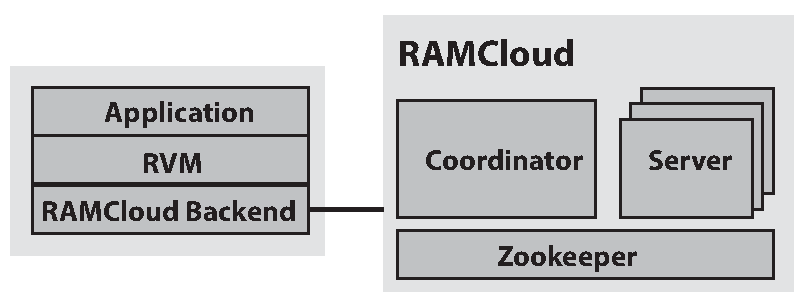
\includegraphics[scale=0.60]{graphs/ramcloud_backend_design2.pdf}
\end{center}
\caption{RAMCloud backend layer operating along side RAMCloud.}
\label{fig:ramcloud_backend_design}
\end{figure}

\begin{figure}[t!]
\begin{center}
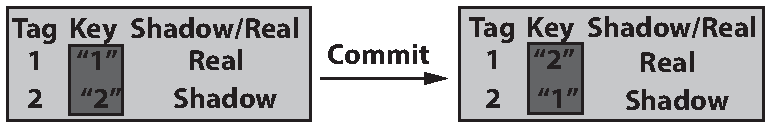
\includegraphics[scale=0.60]{graphs/ramcloud_backend_commit.pdf}
\end{center}
\caption{Diagram of tag/key mapping transformation during commit for a single memory region.}
\label{fig:ramcloud_backend_commit}
\end{figure}

To investigate the performance and suitability of a key-value store as a block device we developed a software layer on top of RAMCloud, a low-latency key-value store.
In RAMCloud, blobs of memory (values) are identified by keys (strings). When running RAMCloud is composed of three main executing instances: a coordinator, a server and Zookeeper (see Figure~\ref{fig:ramcloud_backend_design}).
Each server is responsible for storing and serving data (values). The coordinator is responsible for keeping track of all servers alive and for keeping track of where data is stored in the system.
A Zookeeper instance is used for leader election and for storing configuration data.

Because RAMCloud's data is reference by keys (string) this layer keeps a map structure that associates each tag to a key. This means that each recoverable memory region can be uniquely identified by a key.

To provide atomicity and durability of the tag/key mapping, this backend keeps a special entry in RAMCloud with each tag-key association. This table is read each time the software layer is started and written once for each commit. Because this entry can be atomically written with a {\emph put} operation, we can provide very efficient atomic writes.

Th RMEM's layer operations are implemented in the following way:

\paragraph {\bf Connect} During connection the backend creates a RAMCloud client instance that is responsible for estabilishing a connection to the RAMCloud server.
If this is not the first time this connection is performed, i.e., if the client is under recovery, the backend recoveres each tag-key mapping.
Otherwise, this layer initializes a RAMCloud table and stores an empty master entry in the RAMCloud's server.
\paragraph{\bf Allocate} During allocation, first the backend creates a key that identifies the memory being allocated in the RAMCloud server. Secondly, RAMCloud initializes
\paragraph{\bf Write} To write a memory region (identified by a tag) the backend fetches the tag's corresponding key and issues a {\emph put } operation with that key and corresponding data.
\paragraph{\bf Read} Likewise, to read a memory region the backend issues a {\emph get} operation with the tag's corresponding key. The data read from RAMCloud is copied to the final destination.
\paragraph{\bf Commit} To perform commit, the backend constructs a new master entry where each tag points to the key of the shadow memory being commited (see Figure~\ref{fig:ramcloud_backend_commit}). Likewise, the tag for each of the shadow
memory regions is made to point to the key of the old memory region (rephrase). Once this master entry is constructed in the backend, it is written atomically to RAMCloud.
\paragraph{\bf Disconnect} To disconnect, the backend clears the main data structures (e.g., local tag-key map).

Our design is simplified by the fact that our framework only replicates data to a single node. This means that we do not have to coordinate replicas.

